\chapter{Phân tích và thiết kế hệ thống}
\section{Thu thập dữ liệu}
\subsection{Nguồn dữ liệu}
Poloniex là một sàn giao dịch tiền mã hóa trực tuyến và có trụ sở tại Mỹ. Được 
thành lập vào tháng 1 năm 2014, khi đi vào hoạt động, Poloniex định hướng cung 
cấp một môi trường thương mại an toàn, đồng thời còn cung cấp các dữ liệu về 
thị trường như biểu đồ, bảng xếp hạng và các công cụ phân tích dữ liệu để hỗ 
trợ khách hàng.\\\\
Ngoài ra, Poloniex còn cung cấp một số lượng dữ liệu liên quan đến các thống kê 
mua/bán của sàn giao dịch, các dữ liệu này được cung cấp thông qua API. 
\subsection{Mẫu dữ liệu}
Nguồn dữ liệu được lấy thông qua API dữ liệu biểu đồ thị trường của sàn giao 
dịch Poloniex. Cụ thể API:
\begin{lstlisting}
https://poloniex.com/public?command=returnChartData&currencyPair=BTC_XMR&start=1405699200&end=9999999999&period=14400
\end{lstlisting}
Tập dữ liệu về các phiên giao dịch Bitcoin được thu thập từ ngày 20/2/2015 đến 
ngày 29/10/2016 và có tổng cộng 29634 mẫu (mỗi mẫu là đại diện của một phiên 
giao dịch).
Dữ liệu trả về là một mảng các phần tử JSON có dạng như sau:
\begin{lstlisting}
[
    {"date":1424372400,"high":225,"low":225,"open":225,"close":225,"volume":0.999999,"quoteVolume":0.00444444,"weightedAverage":225},
    {"date":1424374200,"high":225,"low":225,"open":225,"close":225,"volume":0,"quoteVolume":0,"weightedAverage":225},
    ...,
    {"date":1482575400,"high":900.79862142,"low":894.98864451,"open":900.79862142,"close":895.56277339,"volume":2427.10998126,"quoteVolume":2.70065724,"weightedAverage":898.71085649}
]
\end{lstlisting}
Sau khi thu thập, dữ liệu được tiền xử lý để loại bỏ các thông tin không được 
sử dụng trong quá trình phân tích và xây dựng giải thuật. Giá trị có khóa là 
$close$ là dữ liệu sẽ được sử dụng, các giá trị như: $date$, $high$, $low$, 
$open$, $volume$, $quoteVolume$, $weightedAverage$ sẽ được lược bỏ.
\section{Xây dựng MNN}
\subsection{Xây dựng dữ liệu luyện tập}
Một trong những yếu tố hết sức quan trọng trong Máy học đó chính đặc trưng 
- feature. Đặc trưng chính là các giá trị thuộc tính đại diện cho tập dữ liệu 
luyện tập, ví dụ chúng ta có tập dữ liệu về loài chim thì có thể nói đặc trưng 
chính là các thông số như: độ dài sải cánh, màu lông, vùng sinh sống... Một 
giải thuật có thể học được ``kinh nghiệm'' nhanh hay chậm, chính xác hay sai lệch 
phụ thuộc rất nhiều vào yếu tố đặc trưng. Vì vậy quá trình khai phá dữ liệu 
chính là đi tìm kiếm các đặc trưng có ý nghĩa cho giải thuật máy học và là 
công việc hết sức quan trọng.\\\\
Gọi $S$ là đại diện cho một phiên giao dịch, các đặc trưng được xây dựng như 
sau:
\begin{itemize}
    \item 10 feature RDP: $\{ \: loop\{ RDP_1(S_{i+j})\}_i \: \}_j$ Với 
    $i \in [0:9], \: j \in [0:29634]$
    \item 1 feature SO. Với $ j \in [0:29625] $:\\
    \[
        \{ \%K_j = \frac{P(j+9)-L_{10}}{H_{10}-L_{10}} \}_j
    \]
    \item 1 feature ROC. Với $ j \in [0:29625] $:\\ 
    \[
        \{ ROC_{10}(j)= \frac{P(j+9) - P(j)}{P(j)} \}_j
    \]
\end{itemize}
Ở đây, chúng ta chọn mỗi vector đặc trưng được hình thành bởi 10 phiên giao 
dịch. Các giá trị SO và ROC đều được tính trong thời gian là 10 phiên giao dịch.
Sau khi đã có tập luyện tập (tập hợp các vector đặc trưng), ta cần nhãn - label 
để phân lớp tập luyện tập. Nhãn được định nghĩa như sau, nếu giá BTC ở phiên 
thứ 11 lớn hơn phiên thứ 10 thì nhãn sẽ là 1, ngược lại sẽ là 0 (Phiên 11 chính 
là phiên thứ 1 của nhóm 10 phiên liền sau nhóm 10 phiên hiện đang xét).\\
\[
    label_i = \bigg \{ _{0 \quad if \: P_i(10) \: \leq \: P_{i+1}(1)} ^{1 \quad if \: P_i(10) \: > \: P_{i+1}(1)}
\]
Kết quả dữ liệu luyện tập:
\begin{lstlisting}
0 0.06666666666666667 0.016666666666666666 0 0 0 0 0 0 0 0.08444444444444445 1 0
0.06666666666666667 0.016666666666666666 0 0 0 0 0 0 0 0 0.016666666666666666 1 0
...
0.002400968290280231 3.9565217470358025e-9 0.003910087158215986 -0.00045140752064857115 -0.0013329209110243738 0.0008262923440509297 0.018429551716218056 0.003236901952232515 -0.004644611078085971 -0.0016267310238298762 0.018318840535169866 0.7405268424216611 0
\end{lstlisting}
Mỗi hàng đại diện cho một vector đặc trưng và nhãn, chi tiết ở một vector đặc 
trưng 10 giá trị đầu sẽ là 10 đặc trưng $RDP$, 1 giá trị tiếp theo là đặc trưng 
$ROC$, 1 giá trị tiếp theo là đặc trưng $SO$ và 1 giá trị cuối cùng là nhãn.
\subsection{Học giải thuật}
Bên cạnh chạy giải thuật MNN, chúng ta sẽ chạy các giải thuật khác nhằm so sánh 
và đánh giá giải thuật chính. Các giải thuật được chọn để so sánh với giải thuật 
chính: SVM, KNN, LR.\\\\
Các giải thuật được chạy bằng thư viện scikit-learn phiên bản 0.18.0 với các 
tham số được điều chỉnh như sau:
\begin{table}[h]
\begin{tabularx}{\textwidth}{ |l|l|X| }
\hline
Giải thuật & Lớp giải thuật & Tham số điều chỉnh \\
\hline
KNN & neighbors.KNeighborsClassifier & n\_neighbors = 101, weights = "uniform" \\
\hline
LR & linear\_model.LogisticRegression & C = 1 \\
\hline
SVM & svm.SVC & kernel = "linear", C = 1, probability = True\\
\hline
MNN & neural\_network.MLPClassifier & solver = "adam", hidden\_layer\_sizes = (100), activation = "logistic", learning\_rate\_init = 0.001 \\
\hline
\end{tabularx}
\caption{Bảng giải thuật}
\end{table}\\
Tập dữ liệu đưa vào được thay đổi thang độ, tất cả các giá trị được nhân với 
1000 nhằm giúp cho các giá trị nằm trong giới hạn kiểu biến Number của Python, 
việc làm này giúp cho quá trình tính toán của máy tính được nhanh hơn và giảm 
thiểu thời gian chạy giải thuật.
\subsection{Đánh giá giải thuật}
Để đánh giá mức độ ý nghĩa của từng giải thuật, chúng ta sẽ sử dụng 3 tham số 
đánh giá là Accuracy, Recall, Precision. Để có được kết quả đánh giá trên lý 
thuyết, tập dữ liệu sẽ được chia ra thành hai phần:
\begin{itemize}
\item Tập huấn luyện: chiếm 7/10 tổng số dữ liệu, dùng để chạy trong quá trình 
học của giải thuật.
\item Tập đánh giá: chiếm 3/10 tổng số dữ liệu, dùng để chạy trong quá trình 
đánh giá giải thuật.
\end{itemize}
Mô hình đánh giá giải thuật được mô tả bằng cách, dùng tập huấn luyện để tạo 
ra mô hình máy học của các giải thuật, sau đó sử dụng tập đánh giá để làm đầu 
vào cho từng mô hình, kết quả dự đoán sẽ được so sánh với kết quả thực tế của 
từng vector đặc trưng đầu vào. Kết quả so sánh được ghi nhận lại.\\\\
Kết quả chạy giải thuật được xuất ra dưới dạng ma trận nhầm lẫn - confusion 
matrix, sau đó, sử dụng kết quả của ma trận nhầm lẫn để tính toán giá trị của 
các tham số đánh giá. Cụ thể, kết quả của 4 giải thuật được trình bày như sau:
\begin{table}[h]
\centering
\begin{tabular}{ |c|c|c|c|c| }
\hline
 & KNN & LR & SVM & MNN \\
\hline
Accuracy & 62.93\% & 66.24\% & 66.40\% & 69.86\% \\
\hline
Precision & 44.69\% & 18.18\% & 0\% & 60.50\% \\
\hline
Recall & 43.62\% & 0.15\% & 0\% & 29.55\% \\
\hline
\end{tabular}
\caption{Bảng đánh giá}
\end{table}\\
Trước tiên theo bảng đánh giá, ta có các giải thuật LR và SVM cho kết quả Accuracy
là gần khoảng 66\%, nhưng khi nhìn vào chi tiết các giá trị Precision và Recall 
ta nhận thấy kết quả điều cho ra rất thấp. Kết quả này cho thấy giải thuật LR 
và SVM đều có số lần True Positive là xấp xỉ bằng 0, đồng nghĩa với việc các 
giải thuật này hầu như chỉ dự đoán kết quả là nhãn $Down$ cho tất cả trường hợp. 
Điều này hoàn toàn không có ý nghĩa trong dự đoán đầu tư.\\\\
Xét đến KNN và MNN, đối với KNN ta có thể thấy giải thuật có xu hướng cân bằng 
các giá trị Accuracy, Precision và Recall. Nhưng đối với MNN, giải thuật có xu 
hướng tối ưu hóa bộ thiêu chuẩn Accuracy và Precision. Vậy câu hỏi đặt ra ở đây 
là kết quả nào có giá trị đầu tư hơn?\\\\
Chú ý đến Recall, dựa theo định nghĩa thì Recall có thể hiểu nếu trong thực tế 
có 10 phiên là $Up$ thì KNN sẽ dự đoán đúng khoảng 4 lần và MNN sẽ dự đoán đúng 
khoảng 3 lần. Điều này có nghĩa là KNN sẽ chiếm ưu thế so MNN khi sử dụng tiêu 
chuẩn là Recall.\\\\
Xét đến Precision, ta có thể hiểu Precision như sau, với 10 lần dự đoán sẽ có 
phiên $Up$ thì KNN sẽ đúng khoảng 4 lần và MNN sẽ dự đoán đúng 6 lần. Giả sử, 
mức độ tin tưởng của chúng ta vào hệ thống là 100\%, cứ mỗi lần hệ thống dự 
đoán có phiên $Up$ thì ta sẽ quyết định đầu tư. Điều đó đồng nghĩa, nếu theo 
KNN sẽ có 6 lần ta chịu lỗ vì hệ thống dự đoán sai và với MNN thì ta sẽ có 4 
lần ta chịu lỗ.\\\\
Quay lại với Recall, giá trị này không đo đạt được việc chúng ta sẽ lợi nhuận 
hoặc thua lỗ ra sao mà thực ra là giá trị đo đạt khả năng tận dụng cơ hội của 
hệ thống.\\\\
Tới lúc này, ta có thể kết luận, bộ tiêu chuẩn chiếm ưu thế cao hơn sẽ là Accuracy 
và Precision. Điều đó cũng có nghĩa là giải thuật MNN cho kết quả ý nghĩa hơn so 
với KNN và sẽ được lựa chọn để giải quyết bài toán dự đoán xu hướng giá trị BTC.
\section{Xây dựng hệ thống}
Hệ thống được xây dựng với mục tiêu là một ứng dụng nền web, cung cấp công cụ hỗ 
trợ cho việc dự đoán xu hướng giá trị BTC.
\subsection{Tổng quan hệ thống}
Hệ thống được xem xét và được thiết kế với 3 khối máy chủ , mỗi khối máy chủ đại 
diện cho một khối chức năng riêng biệt. Cấu trúc hệ thống như vậy nhằm dự trù và đảm bảo 
cho các hoạt động về quản lý hệ thống như phân phối tải, bảo trì và mở rộng sau 
này được thực hiện dễ dàng và tiết kiệm thời gian. Chi tiết các hệ thống máy chủ:
\begin{itemize}
\item Hệ thống máy chủ máy học - Machine Learning server
\item Hệ thống máy chủ backend - Backend server
\item Hệ thống máy chủ UI frontend - UI Frontend server
\end{itemize}
Các khối hệ thống giao tiếp với nhau bằng API và Socket - đối với các chức năng
chạy thời gian thực.\\
\begin{figure}[h!]
\centering
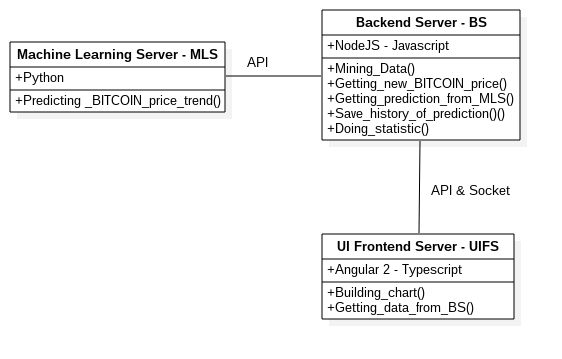
\includegraphics[height=3.5in, keepaspectratio=true]{system.png}
\caption{Cấu trúc quan hệ và chức năng hệ thống}
\end{figure}
\subsection{Hệ thống máy chủ máy học}
Đây là hệ thống cốt lõi của của sản phẩm, nó đảm nhiệm khối chức năng chính 
liên quan đến các tác vụ máy học, cụ thể, dựa vào các tham số được truyền vào 
để thực hiện quá trình chạy giải thuật dự đoán từ đó đưa ra giá trị nhãn dự 
đoán tương ứng cho bộ tham số đó.\\\\
Lưu ý, để đưa ra một kết quả dự đoán, hệ thống yêu cầu các tham số đầu vào phải 
được xây dựng theo mô tả tại mục 4.1.1 với tổng số đặc trưng là 12.\\\\
Hệ thống máy chủ máy học được chia thành hai phần:
\begin{enumerate}
\item Prediction: bao gồm các chức năng đọc mô hình MNN đã xây dựng, chạy mô 
hình với tham số truyền vào và lấy các kết quả đầu ra.Kết quả đầu ra có giá 
trị nhãn $Up-Down$ và xác suất dự đoán.
\item Django: bao gồm các chức năng để trở thành một máy chủ giao tiếp thông 
qua API, các chức năng có thể ví dụ như tiếp nhận các yêu cầu thông qua API, 
phản hồi các yêu cầu dưới dạng các kết quả JSON...
\end{enumerate}
Vì tính chất hỗ trợ tốt cho Máy học nên Python được lựa chọn là ngôn ngữ để 
phát triển hệ thống này.
\subsection{ Hệ thống máy chủ backend}
Vì bản thân hệ thống máy chủ máy học không có các khối chức năng liên quan đến 
việc lấy dữ liệu giá BTC cũng như khai phá dữ liệu, nên hệ thống máy chủ backend 
được xây dựng để thực hiện các chức năng này. Đồng thời, máy chủ backend còn là 
cầu nối giữa trải nghiệm người dùng (hệ thống máy chủ UI frontend) và hệ thống 
máy chủ máy học.\\\\
Để thực hiện được công việc trên, hệ thống bao gồm được xây dựng các chức năng:
\begin{enumerate}
\item Cập nhật giá BTC: thông qua các public API được sàn giao dịch Poloniex 
cung cấp, các hàm lấy giá được chạy liên tục để cập nhật giá BTC mới nhất nhằm 
phục vụ cho quá trình dự đoán (trung bình 20 giây).
\item Khai phá dữ liệu: dữ liệu được các hàm cập nhật giá BTC lấy được vẫn 
còn ở dạng thô, chưa qua xử lý. Khai phá dữ liệu là biến đổi các dữ liệu này 
về các bộ tham số có ý nghĩa với Máy học, các giá trị này mới đích thực 
dùng để làm đầu vào dự đoán xu hướng giá trị BTC.
\item Giao tiếp với hệ thống máy chủ máy học: truyền tham số đi và nhận 
kết quả trả về từ hệ thống máy chủ máy học thông qua API.
\item Lưu trữ và thống kê dữ liệu: thực hiện việc lưu trữ dữ liệu, từ đó tạo 
nên một hệ thống các dữ liệu phục vụ cho việc phân tích, thống kê để cung cấp 
cho người dùng đầu cuối. Đó là các thông tin hết sức quý giá phục vụ cho các 
nhà đầu tư.
\item Giao tiếp với hệ thống máy chủ UI frontend: đưa ra những API chức năng 
nhằm phục vụ cho máy chủ UI frontend. Ví dụ như: yêu cầu dữ liệu dự đoán, yêu 
cầu thống kê đúng/sai, yêu cầu dữ liệu giá cho biểu đồ...
\end{enumerate}
Với khả năng xử lý nhanh, được hỗ trợ tốt nên NodeJS được dùng để phát triển 
hệ thống. Đồng thời, cơ sở dữ liệu của hệ thống là MongoDB vì tính linh hoạt 
trong cấu trúc dữ liệu và khả năng mở rộng cao.
\subsection{Hệ thống máy chủ UI frontend}
Hệ thống máy chủ UI frontend là một giao diện người dùng, nó cho phép người 
dùng có thể tiếp cận với các chức năng của toàn bộ hệ thống một cách dễ dàng. 
Hệ thống bao gồm nhiều biểu đồ, cũng như tham số cung cấp các thông tin có ý 
nghĩa đầu tư - dự đoán xu hướng giá trị Bitcoin - đồng thời với đó, là các 
thông tin về độ tin cậy của hệ thống, các thống kê về lịch sử dự đoán...\\\\
Một số hình ảnh về hệ thống thực tế.\\
\begin{figure}[h!]
\centering
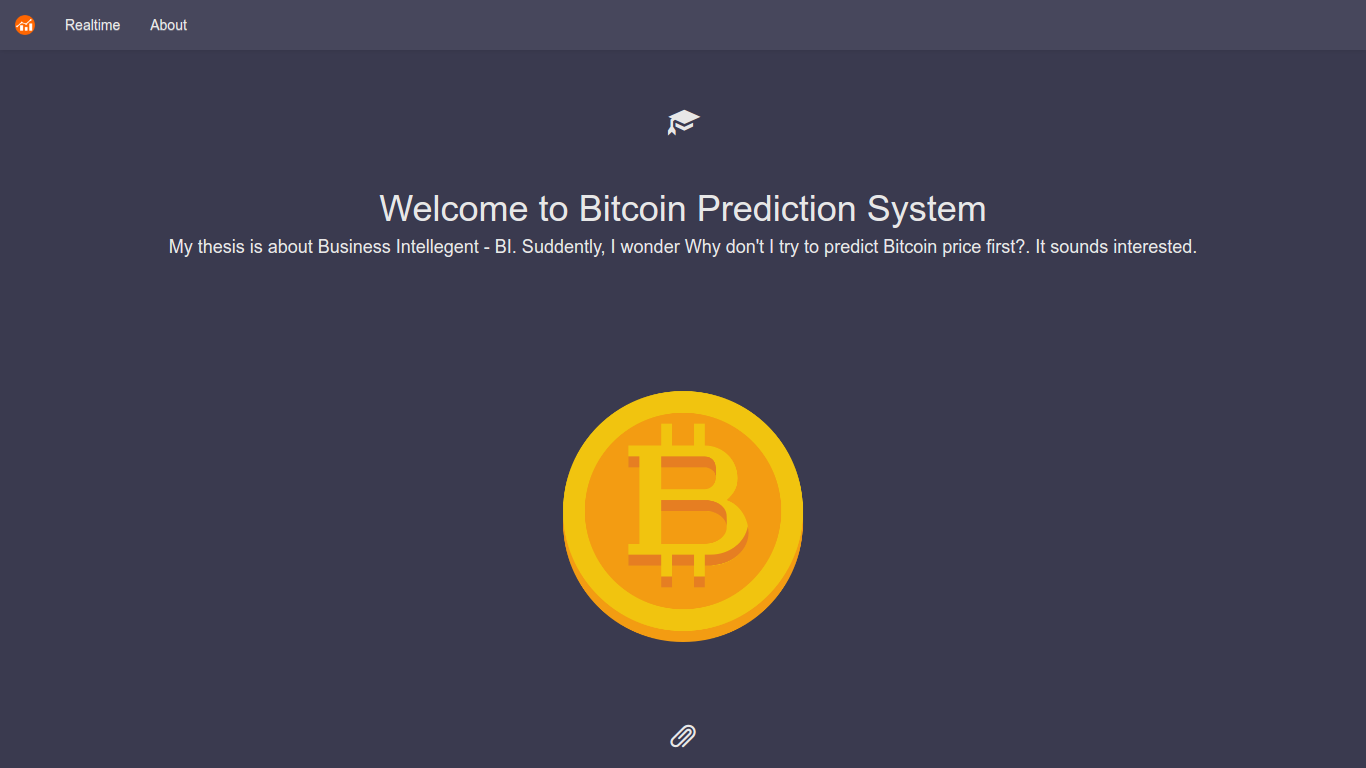
\includegraphics[height=3in, keepaspectratio=true]{1.png}
\caption{Giao diện 1 máy chủ UI frontend}
\end{figure}\\
\begin{figure}[h!]
\centering
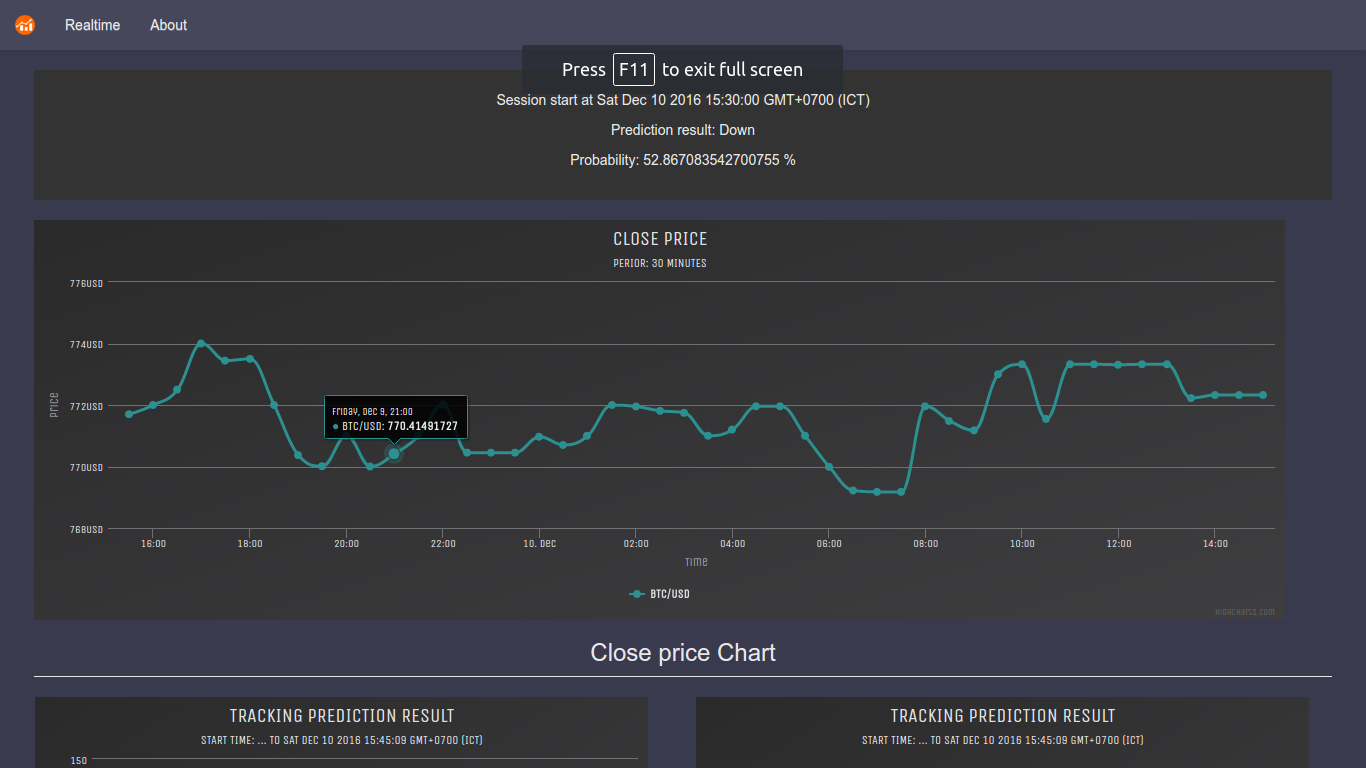
\includegraphics[height=3in, keepaspectratio=true]{2.png}
\caption{Giao diện 2 máy chủ UI frontend}
\end{figure}\\\\
\begin{figure}[h!]
\centering
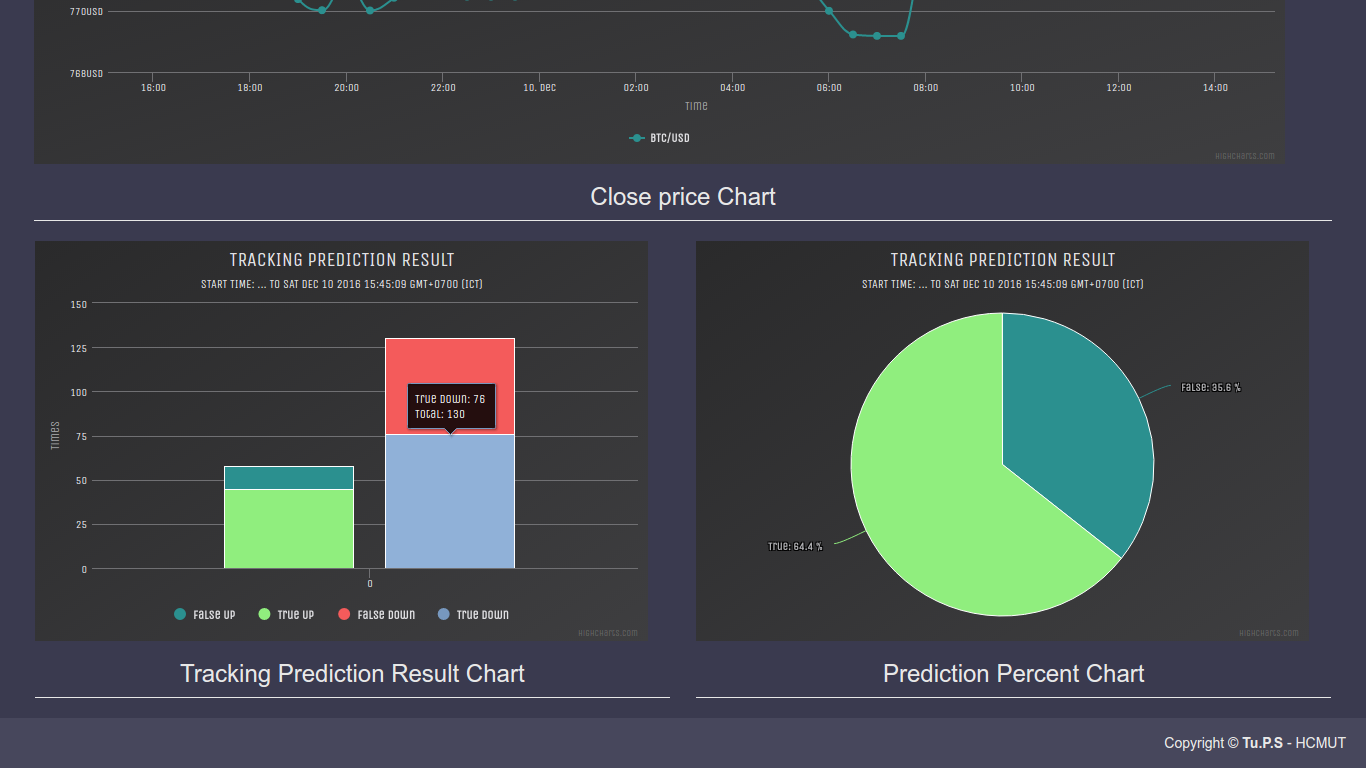
\includegraphics[height=3in, keepaspectratio=true]{3.png}
\caption{Giao diện 3 máy chủ UI frontend}
\end{figure}\\\\
Hệ thống máy chủ UI frontend được xây dựng theo xu hướng one-page, cũng chính 
vì vậy mà Angular 2 là lựa chọn phù hợp, với khả năng phát triển nhanh, hỗ trợ 
tốt từ các bên thứ 3.